\documentclass[12pt]{article}
\usepackage{amsmath}
\usepackage{amssymb}
\usepackage{enumitem}
\usepackage{geometry}
\usepackage{setspace}
\usepackage{makecell}
\usepackage{multirow}
\usepackage{graphicx}

\usepackage{listings}
\lstset{
    basicstyle=\footnotesize\ttfamily,
    numbers=left,
    stepnumber=1,
    showstringspaces=false,
    tabsize=1,
    breaklines=true,
    breakatwhitespace=false
}
\geometry{margin=1in}

\begin{document}
\doublespacing
\setlength{\abovedisplayskip}{-10pt}
\setlength{\belowdisplayskip}{-10pt}
\setlength{\abovedisplayshortskip}{0pt}
\setlength{\belowdisplayshortskip}{0pt}

\vspace*{\fill}
\begin{center}
\textbf{Final Assignment}
\end{center}
\quad
\begin{center} Abhinav Inavolu, Ivan Mladenov \end{center}
\begin{center} Advanced Cybersecurity Experience for Students, University of Maryland College Park \end{center}
\begin{center} HACS 101: Applied Cybersecurity Foundations \end{center}
\begin{center} Dr. Michel Cukier \end{center}
\begin{center} May 9, 2024 \end{center}
\vfill % equivalent to \vspace{\fill}


\section*{\normalsize{The Honeypot}}
This project aims to set up a high-interaction honeypot to detect what data modern attackers are interested in harvesting. Honeypots will help us answer this question because they can quickly be deployed with modified filesystems with different forms of data for hackers to sift through. Gathering attacker data can help identify their origins and intentions, and help prevent future attacks.  Cleverly designed honeypots can attract hackers and may lead “hackers [to give] away many of their most precious secrets” and oftentimes they have “inadvertently revealed the hacking tools they use and how they use them and what they do when they break into a system” (Burgess, 2023). Specifically, these examples show how high-interaction honeypots are effective because they can gather a genuine representation of what data hackers are targeting and how they interact with vulnerable systems. \newline
\indent We’ll have a control group honeypot that contains very minimal personal data. As we move up the honeypots, the data can grow into more sensitive data (medical, financial, beyond personal data, etc.) which will be stored in a MySQL database to look more realistic. The goal of using an actual database rather than storing all data in random files is to lure attackers into engaging with the system, have them try to exploit/attack the SQL server, and see what they do with the data afterward. \newline
\indent Suppose we learn which honey is most attractive. In that case, future honeypots can be set up to collect more data about hackers, giving cybersecurity teams more opportunities to analyze pattern behaviors from malicious actors or bot attacks. Our goal is to discover which of these honeys will be most effective in capturing and engaging hackers, eventually learning their attack strategies. 


\section*{\normalsize{Technologies}}
\indent This project utilized many topics covered in HACS 101 including containers, networking, Linux services, firewalls, task scheduling, keyloggers, and man-in-the-middle. \newline
\indent The purpose of using a container is to isolate the attackers inside the honeypot and protect the host machine. While virtual machines are also an attractive option, they are much heavier than containers as they have their kernel. A comparative study from computer science researchers from institutions including Georgia Tech and Yunnan University also noted that “primary motivations for the enterprise to adopt the container technology include its convenience to encapsulate and deploy applications, lightweight operations” (Zhang et al., 2018). Our containers will allow us to quickly spawn new honeypots, randomize them, and configure them with the necessary data to attract new attackers. Once we’re satisfied with the data from the honeypot, we can also quickly destroy and redeploy after we’ve collected and analyzed the hackers’ activity. \newline
\indent To route attacker traffic into our honeypot, we set up our firewall program such that incoming connections route to our container. For this honeypot, we are using the \textit{iptables} firewall program and Network Address Translation (NAT) rules to redirect all incoming attacker traffic to the container. The attacker will believe that it’s connected to a server running a database with critical information, when in reality they are sitting in an isolated container inside the actual host machine, with their every move being monitored. \newline
\indent We'll rely on a few key Linux services to spawn the containers and turn them into honeypots. For starters, we’ll use the Linux Container (LXC) service to create, set up, and destroy all our honeypots. Also, to allow attackers in, we can attach to the honeypots with LXC and install another service called OpenSSH. Setting up the SSH server on the container will enable hackers to or bots looking to connect to remote machines to connect to our server and get stuck in the honeypot. Finally, we’ll use the MySQL service to run an SQL database server to store our honey realistically. By keeping this server running, it makes the honeypot more believable and interactive as the hacker can try poking through the database and cracking into it to get sensitive information. This is where our data variation will occur, and different levels of honey will be added to determine which ones the hacker will be more invested in. \newline
\indent Task scheduling will also be an important part of maintaining the honeypot because we must continuously harvest, organize, and clear out log files from the containers. We’ll use task scheduling scripts to collect data from the Man-in-the-middle tracking and logs from our Snoopy keylogger, which will be explained further below. \newline
\indent Our host machine will run a Javascript program that launches a man-in-the-middle server that intercepts SSH traffic between the hacker and the honeypot container. By doing so, we can collect the commands the attacker enters through the log files that the program runs and analyze the hacker’s behavior. This program also allows us to track how long the hacker was in the container and the extent of the hacker’s engagement with the database and exploring our honeypot. \newline
\indent The last component of the honeypot is to log every keystroke that the hacker inputs so that we can dive deeper into monitoring their exact behavior and patterns. We’ll achieve this by installing the Snoopy keylogger onto our container, which will store all the hacker’s keystrokes into a log file which we can then copy back to the host for processing. \newline
\indent An important note to make is that despite learning about these topics in HACS101, we will not be relying on any port-scanning technologies or packet capture to run our honeypot. Port scanning isn't a large concern on our end because we are deliberately exposing the SSH port to our machine so that hackers can enter into our system. While hackers may be using port scanners to find available ports on our host machine, we will not be making use of these tools because we're the ones hosting the vulnerable container. Similarly, we aren't capturing any outgoing packets on the container as we are more focused on gathering the commands and keystrokes of the hacker rather than the data that they are trying to send in or out of our container. 


\section*{\normalsize{Design}}
\indent To set up the honeypot’s system and network configuration, we need to use the Linux services mentioned above to place the honey in the container and route hackers from our host directly into our container. We’ll do this by setting up the firewall with the aforementioned \textit{iptables} command, using pre- and postrouting rules to direct any incoming traffic to the internal IP address of the container. At the top of our \textit{iptables}, we must also insert a rule that routes SSH traffic specifically through our MITM server so we can collect the commands. \newline
\indent Another one of the aforementioned Linux services that we’ll rely on is MySQL, which will help us convincingly store the data. We’ll launch a database and insert some personal information into the tables for the hacker to look for. \newline
\indent To collect our data, we’ll copy over the data from our Snoopy keylogger running on the honeypot container. To do this recurrently and periodically, we can schedule a \textit{cronjob} to do this for us on given timestamps. We’ll then move those files into a folder on the host machine to keep track of our logs and clean up the file on the container to prevent it from holding an excessive amount of data at once (or else it would be unreadable and difficult to analyze). \newline
\indent We will utilize three different types of honey to analyze which one attackers are most interested in: minimal personal data, medical data, or financial data. All three data sets will be stored in a MySQL server to make the honeypot more convincing. The data sets will be generated using Python scripts that pull data from free APIs such as the Google Maps API. We will use data from these APIs in conjunction with other data points randomly generated to produce .csv files storing the data. These .csv files will then be fed into the MySQL server.


\section*{\normalsize{Implementation}}
\indent To set up the honeypot, we’ll have a main script called \textit{honeypot.sh} which sets up an Ubuntu container. The script will also install all the important binaries we need for the services and keyloggers mentioned above, including the MySQL database. After those services are up and running, we can place the data into the MySQL database for the attacker to find. This will be done by redirecting an SQL file (named \textit{database.sql}) with the necessary personal information (for this simple demo we just placed our names and addresses into it) as input to the \textit{mysql} command. The final steps in the script will be to set up the firewall and immediately launch the MITM server. \newline
\begin{center} 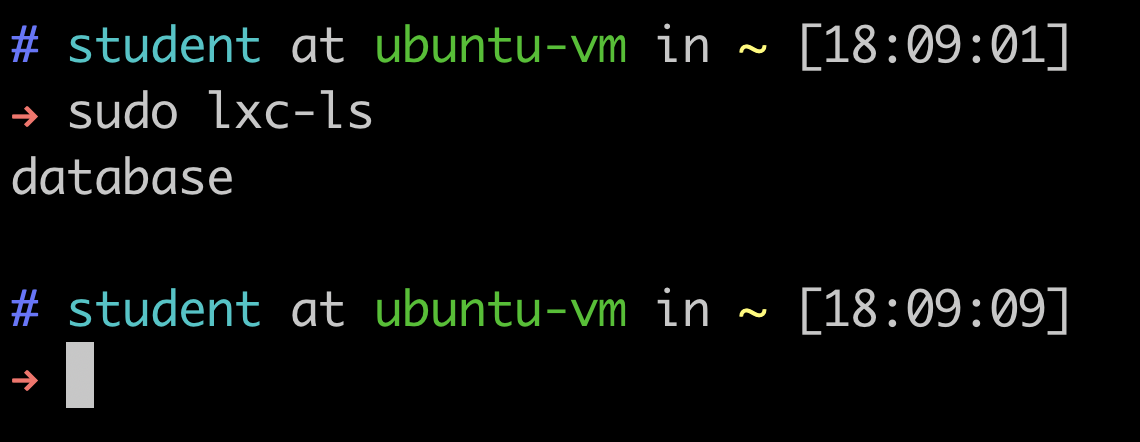
\includegraphics[scale=0.5]{./container.png} \end{center}
\begin{center} \textit{Running Container after Setup Script} \end{center}
\begin{center} 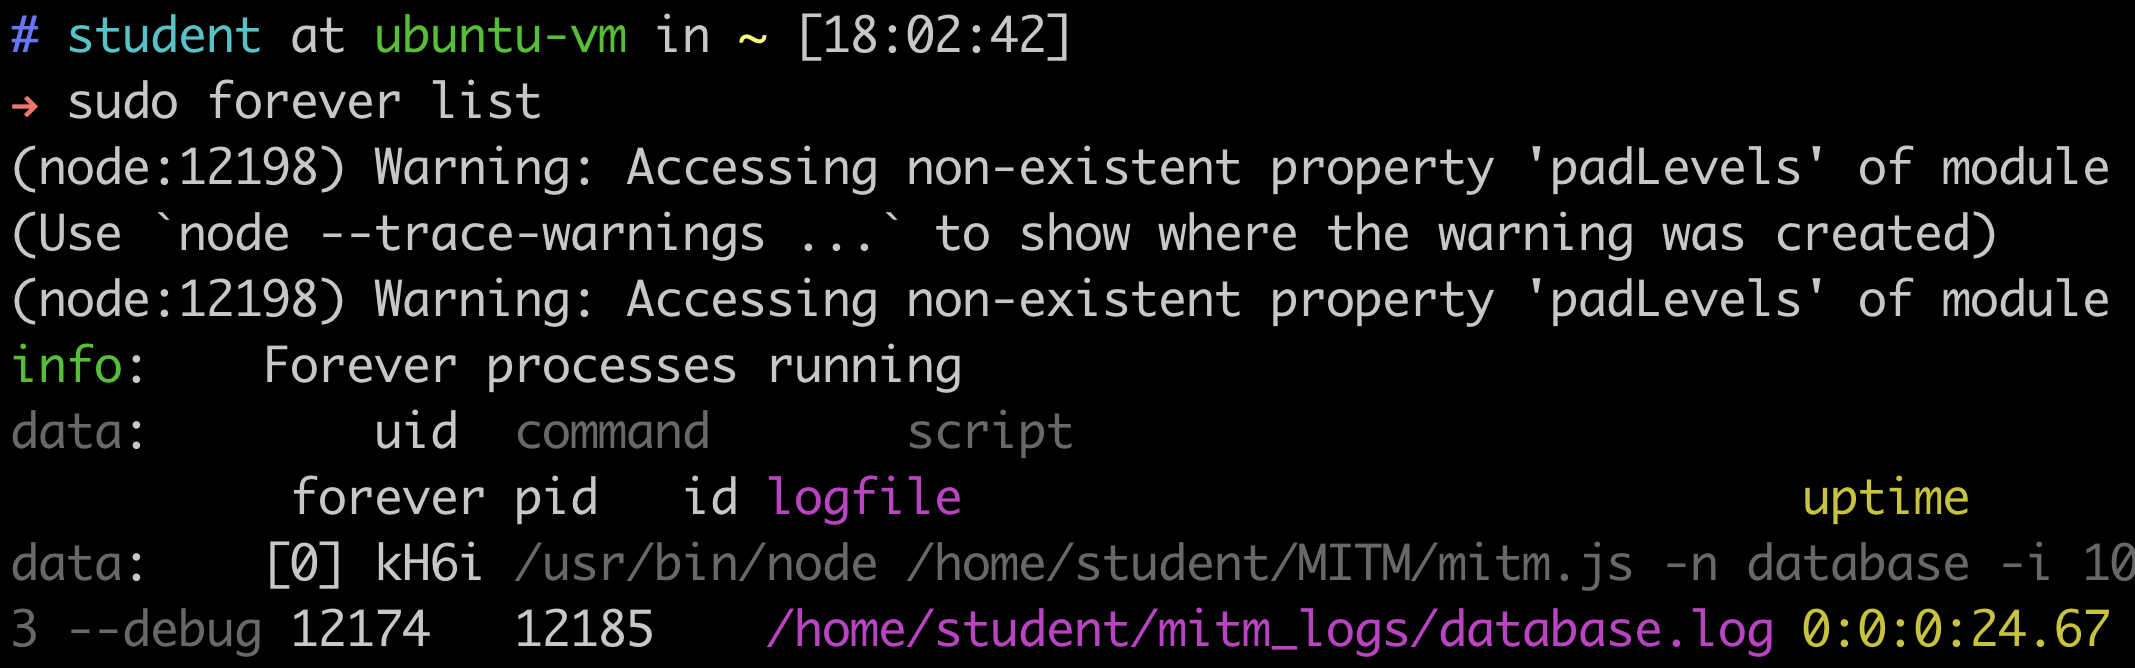
\includegraphics[scale=0.25]{./mitm.png} \end{center}
\begin{center} \textit{Running MITM Server on Host} \end{center}
\begin{center} 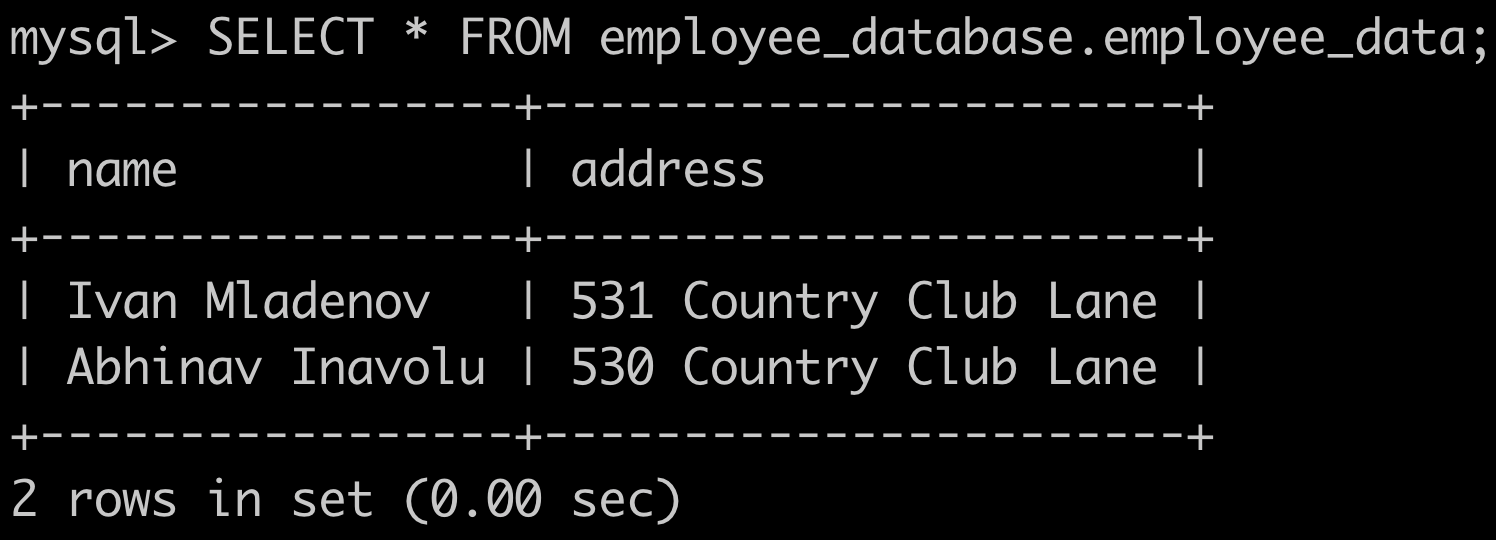
\includegraphics[scale=0.5]{./mysql.png} \end{center}
\begin{center} \textit{Database with Sample Minimal Data} \end{center}
\qquad The honeypot script takes care of most of the important setup, so the only other script we’ll rely on is a cleanup script that will copy over log data generated by Snoopy. This \textit{clean.sh} script will copy over the log file into a folder of files that name the logs based on the date they were copied over, and then clear out the log file on the container so that it can collect fresh data. The final step is to schedule this script so that it runs frequently, in our case once daily. We’ll do this by placing a rule at the bottom of our host machine’s crontab so that it can run the \textit{clean.sh} script every day. \newline
\begin{center} 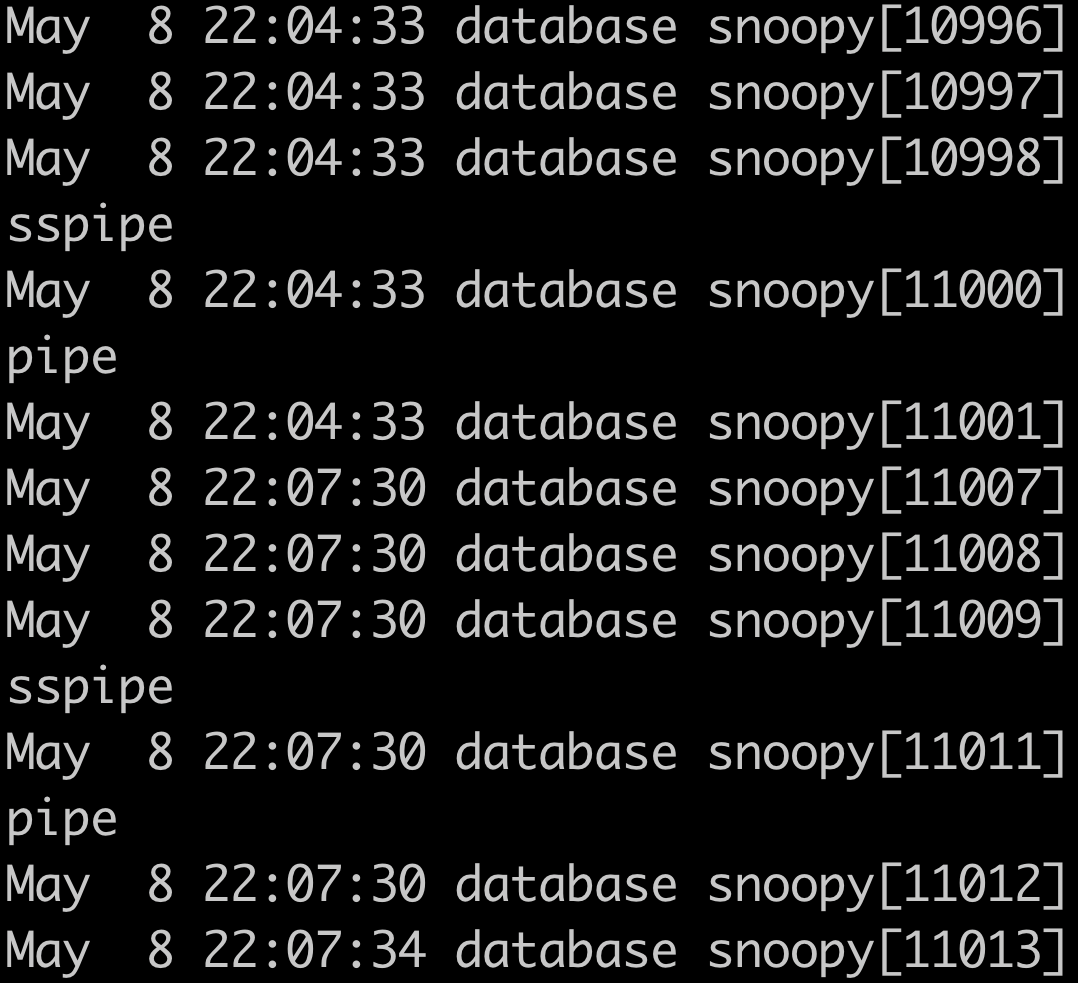
\includegraphics[scale=0.5]{./snoopy.png} \end{center}
\begin{center} \textit{Sample Log Output from Snoopy} \end{center}
\begin{center} 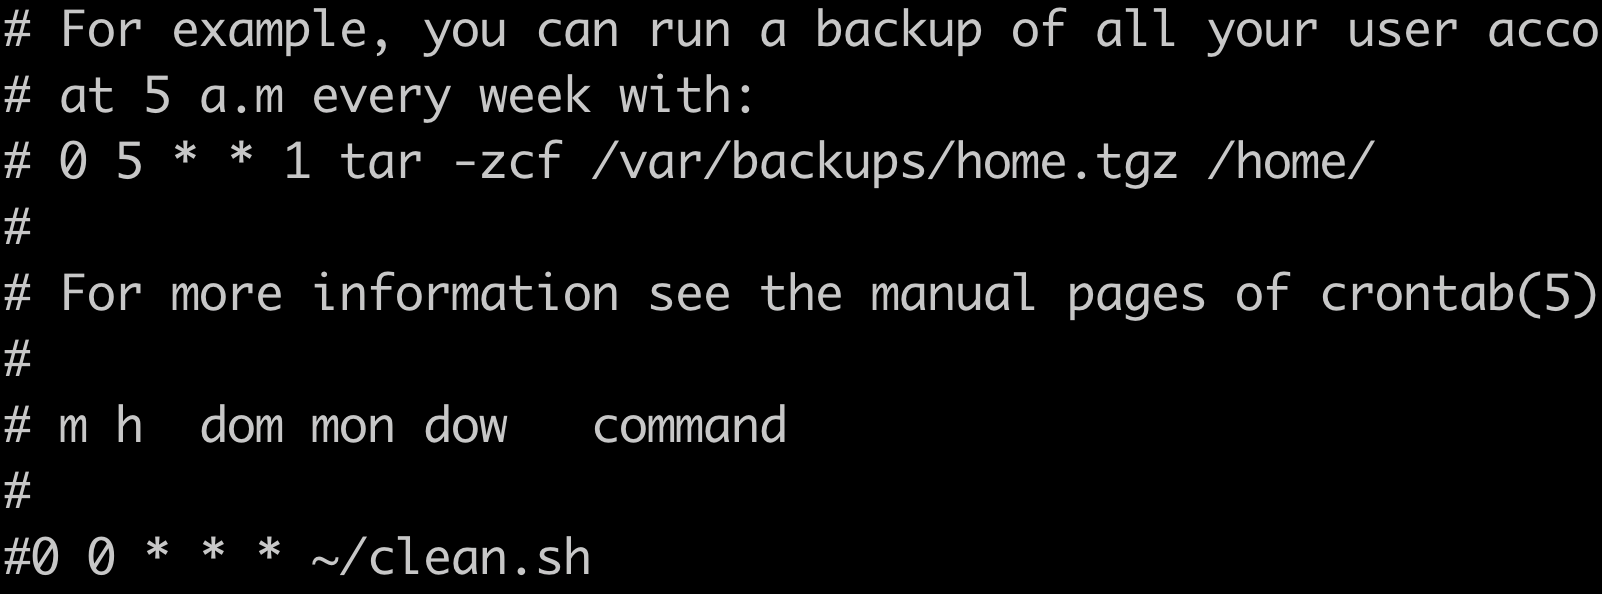
\includegraphics[scale=0.5]{./crontab.png} \end{center}
\begin{center} \textit{Updated Crontab with Clean Script} \end{center}
\qquad The scripts and database files mentioned above will be placed in the Appendix for reference. 


\section*{\normalsize{Data Analysis}}
\indent The three metrics we plan on using to measure attacker engagement will be the mean amount of time the attackers spent logged in, the mean number of keystrokes, and the mean number of commands run. \newline
\indent The two statistical analysis methods we plan on using are the Kruskal-Wallis test, a method to find statistically significant differences in three or more sample medians, and the Mann-Whitney U Test, a method to find if two samples have statistically significant differences (Kruskal \& Wallis, 1952; Mann \& Whitney, 1947). \newline
\indent If the differences in metrics are statistically significant, we will use the median values produced by the Kruskal-Wallis test to help rank the honeys in order of attacker engagement. We will then use the Mann-Whitney U test to determine whether any of the honeys were tied with each other in terms of attacker engagement. The analysis will be done with R since it has both the Kruskal-Wallis test and the Mann-Whitney test built-in. Below is an example of our analysis with some example data using a significance level of $\alpha=0.05$. \newline 
\begin{table}[h!]
\begin{tabular}{|ccccccccc|}
\hline
\multicolumn{9}{|c|}{Example Data}                                                                                                                                                                                                                                                    \\ \hline
\multicolumn{3}{|c|}{Minimal Data}                                                                 & \multicolumn{3}{c|}{Medical Data}                                                                 & \multicolumn{3}{c|}{Financial Data}                                          \\ \hline
\multicolumn{1}{|c|}{\makecell{Time\\(min)}} & \multicolumn{1}{c|}{Keystrokes} & \multicolumn{1}{c|}{\makecell{Com-\\mands}} & \multicolumn{1}{c|}{\makecell{Time\\(min)}} & \multicolumn{1}{c|}{Keystrokes} & \multicolumn{1}{c|}{\makecell{Com-\\mands}} & \multicolumn{1}{c|}{\makecell{Time\\(min)}} & \multicolumn{1}{c|}{Keystrokes} & \makecell{Com-\\mands} \\ \hline
\multicolumn{1}{|c|}{28}         & \multicolumn{1}{c|}{1056}       & \multicolumn{1}{c|}{78}       & \multicolumn{1}{c|}{34}         & \multicolumn{1}{c|}{1353}       & \multicolumn{1}{c|}{82}       & \multicolumn{1}{c|}{90}         & \multicolumn{1}{c|}{2319}       & 268      \\ \hline
\multicolumn{1}{|c|}{35}         & \multicolumn{1}{c|}{1462}       & \multicolumn{1}{c|}{90}       & \multicolumn{1}{c|}{49}         & \multicolumn{1}{c|}{1782}       & \multicolumn{1}{c|}{118}      & \multicolumn{1}{c|}{67}         & \multicolumn{1}{c|}{1849}       & 213      \\ \hline
\multicolumn{1}{|c|}{46}         & \multicolumn{1}{c|}{1549}       & \multicolumn{1}{c|}{123}      & \multicolumn{1}{c|}{31}         & \multicolumn{1}{c|}{1192}       & \multicolumn{1}{c|}{93}       & \multicolumn{1}{c|}{103}        & \multicolumn{1}{c|}{2849}       & 295      \\ \hline
\multicolumn{1}{|c|}{24}         & \multicolumn{1}{c|}{1178}       & \multicolumn{1}{c|}{80}       & \multicolumn{1}{c|}{52}         & \multicolumn{1}{c|}{1648}       & \multicolumn{1}{c|}{124}      & \multicolumn{1}{c|}{87}         & \multicolumn{1}{c|}{2103}       & 286      \\ \hline
\multicolumn{1}{|c|}{31}         & \multicolumn{1}{c|}{1336}       & \multicolumn{1}{c|}{88}       & \multicolumn{1}{c|}{51}         & \multicolumn{1}{c|}{1492}       & \multicolumn{1}{c|}{111}      & \multicolumn{1}{c|}{130}        & \multicolumn{1}{c|}{3392}       & 358      \\ \hline
\multicolumn{1}{|c|}{35}         & \multicolumn{1}{c|}{1604}       & \multicolumn{1}{c|}{115}      & \multicolumn{1}{c|}{44}         & \multicolumn{1}{c|}{1284}       & \multicolumn{1}{c|}{79}       & \multicolumn{1}{c|}{88}         & \multicolumn{1}{c|}{2392}       & 257      \\ \hline
\multicolumn{1}{|c|}{19}         & \multicolumn{1}{c|}{824}        & \multicolumn{1}{c|}{67}       & \multicolumn{1}{c|}{38}         & \multicolumn{1}{c|}{1038}       & \multicolumn{1}{c|}{86}       & \multicolumn{1}{c|}{95}         & \multicolumn{1}{c|}{2531}       & 283      \\ \hline
\multicolumn{1}{|c|}{40}         & \multicolumn{1}{c|}{1083}       & \multicolumn{1}{c|}{101}      & \multicolumn{1}{c|}{40}         & \multicolumn{1}{c|}{1270}       & \multicolumn{1}{c|}{95}       & \multicolumn{1}{c|}{116}        & \multicolumn{1}{c|}{2834}       & 323      \\ \hline
\end{tabular}
\end{table}
\clearpage
\begin{align*} 
	H=(N-1)\frac{\sum\limits_{i=1}^g n_{i}(\bar{r}_{i\cdot}-\bar{r})^2}{2} \\
	\textit{Kruskal-Wallis Test Statistic} \\ 
\end{align*}
\begin{table}[h!]
\begin{tabular}{|cccccl|}
\hline
\multicolumn{6}{|c|}{Kruskal-Wallis Test}                                                                                                                                                                                                           \\ \hline
\multicolumn{1}{|c|}{\multirow{2}{*}{}} & \multicolumn{3}{c|}{Sum of Ranks}                                                                           & \multicolumn{1}{c|}{\multirow{2}{*}{\makecell{Kruskal Wallis\\H Statistic}}} & \multirow{2}{*}{p-value} \\ \cline{2-4}
\multicolumn{1}{|c|}{}                  & \multicolumn{1}{c|}{Minimal Data} & \multicolumn{1}{c|}{Medical Data} & \multicolumn{1}{c|}{Financial Data} & \multicolumn{1}{c|}{}                                            &                          \\ \hline
\multicolumn{1}{|c|}{Time (min)}        & \multicolumn{1}{c|}{49}           & \multicolumn{1}{c|}{87}           & \multicolumn{1}{c|}{164}            & \multicolumn{1}{c|}{17.165}                                      & 0.00019                  \\ \hline
\multicolumn{1}{|c|}{Keystrokes}        & \multicolumn{1}{c|}{60}           & \multicolumn{1}{c|}{76}           & \multicolumn{1}{c|}{164}            & \multicolumn{1}{c|}{15.68}                                       & 0.00039                  \\ \hline
\multicolumn{1}{|c|}{Commands}          & \multicolumn{1}{c|}{61}           & \multicolumn{1}{c|}{75}           & \multicolumn{1}{c|}{164}            & \multicolumn{1}{c|}{15.605}                                      & 0.00041                  \\ \hline
\end{tabular}
\end{table}
\quad \newline
\begin{align*}
	U_{1}=n_{1}n_{2}&+{\tfrac {n_{2}(n_{2}+1)}{2}}-R_{2},U_{2}=n_{1}n_{2}+{\tfrac {n_{1}(n_{1}+1)}{2}}-R_{1} \\
	&\textit{Mann-Whitney U Test Statistic}
\end{align*}
\quad \newline
\begin{table}[h!]
\begin{center}
\begin{tabular}{|ccccc|}
\hline
\multicolumn{5}{|c|}{Mann-Whitney U Test}                                                                                                                \\ \hline
\multicolumn{1}{|c|}{\multirow{2}{*}{}} & \multicolumn{2}{c|}{Minimal and Medical Data}                & \multicolumn{2}{c|}{Medical and Financial Data} \\ \cline{2-5} 
\multicolumn{1}{|c|}{}                  & \multicolumn{1}{c|}{z-score}  & \multicolumn{1}{c|}{p-value} & \multicolumn{1}{c|}{z-score}      & p-value     \\ \hline
\multicolumn{1}{|c|}{Time (min)}        & \multicolumn{1}{c|}{-1.94289} & \multicolumn{1}{c|}{0.05238} & \multicolumn{1}{c|}{3.30816}      & 0.00094     \\ \hline
\multicolumn{1}{|c|}{Keystrokes}        & \multicolumn{1}{c|}{-0.78766} & \multicolumn{1}{c|}{0.42952} & \multicolumn{1}{c|}{3.30816}      & 0.0094      \\ \hline
\multicolumn{1}{|c|}{Commands}          & \multicolumn{1}{c|}{-0.68264} & \multicolumn{1}{c|}{0.49650} & \multicolumn{1}{c|}{3.30816}      & 0.0094      \\ \hline
\end{tabular}
\end{center}
\end{table}

\begin{center} 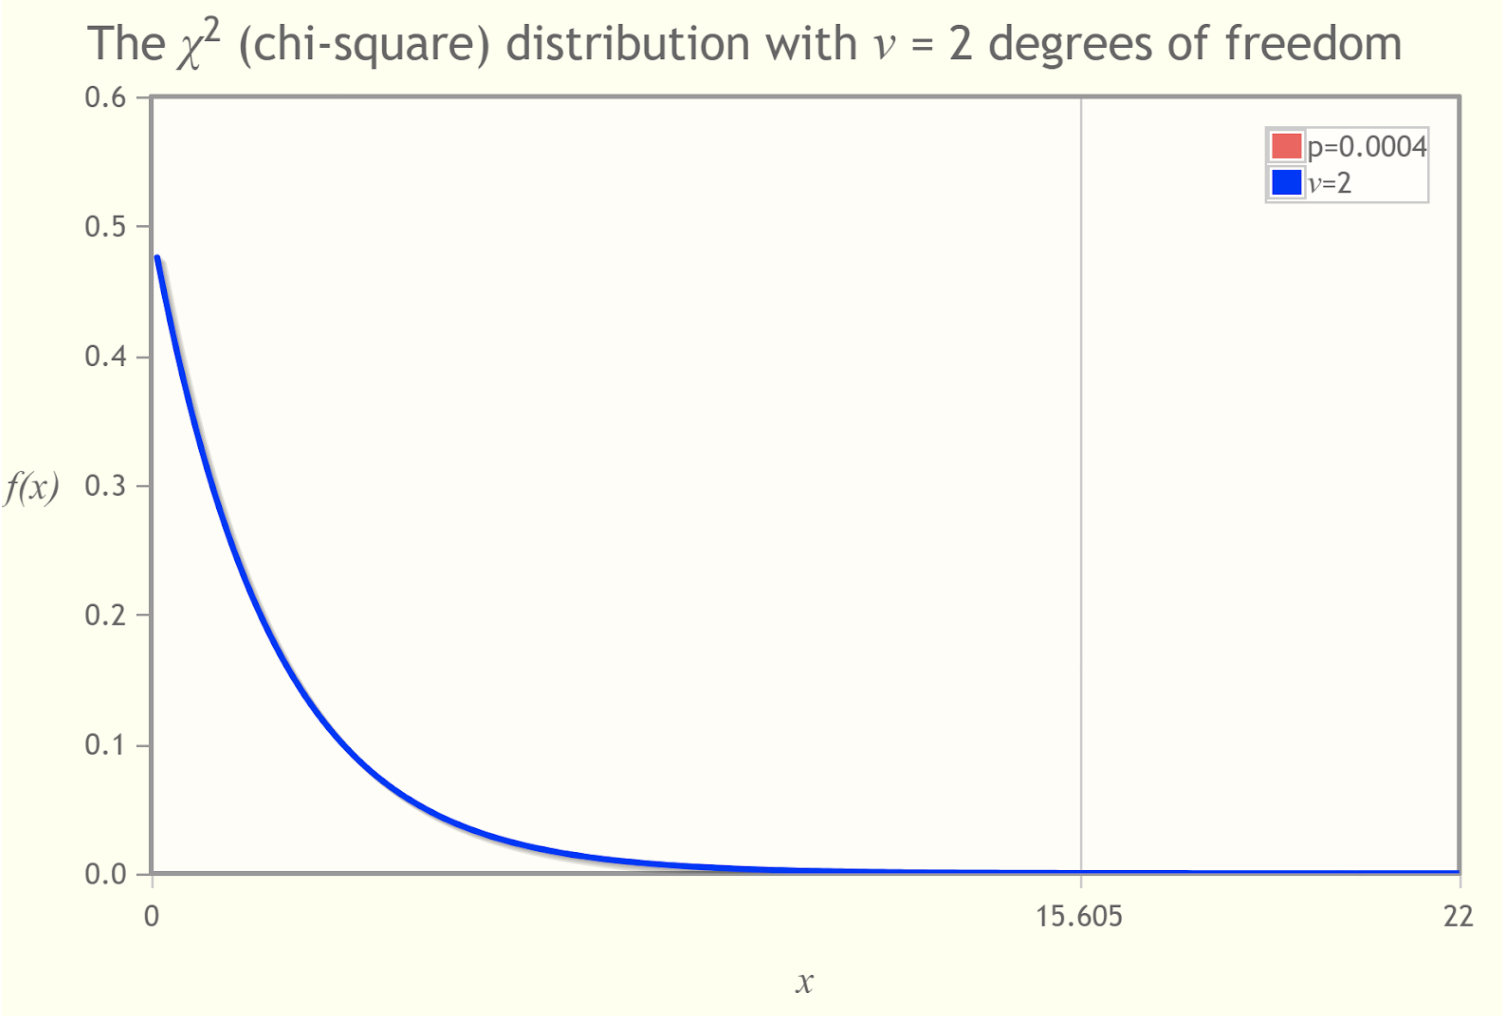
\includegraphics[scale=0.3]{./chi-square.png} \end{center}
\begin{center} \textit{$\chi^2$-Distribution for Commands Run} \end{center}


\indent Based on the rankings from the Kruskal-Wallis test, it initially seems like the financial data had the highest attacker engagement followed by the medical data and then the minimal data. Upon further analysis using the Mann-Whitney U Test however, we realize there is no statistically significant difference between the medical and minimal data while there is a statistically significant difference between the medical and financial data. Based on the results from both tests we can conclude that financial data had the highest attacker engagement while minimal and medical data were tied after financial data. \newline


\clearpage
\begin{center} \section*{\normalsize{Appendix}} \end{center}
\singlespacing
\begin{lstlisting}[caption={honeypot.sh},language={bash}]
#!/bin/bash

# Launch the "database" honeypot
sudo lxc-create -n database -t download -- -d ubuntu -r focal -a amd64
sudo lxc-start -n database
sleep 10

# Fetch the internal IP and store it for routing
IP=$(sudo lxc-info -n database -iH)

# Install important binaries on the honeypot
sudo lxc-attach -n database -- bash -c "sudo apt-get update"
sudo lxc-attach -n database -- bash -c "sudo apt-get install openssh-server -y"
sleep 10
sudo lxc-attach -n database -- bash -c "sudo systemctl enable ssh --now"
sudo lxc-attach -n database -- bash -c "sudo apt-get install wget -y"
sleep 10
sudo lxc-attach -n database -- bash -c "sudo apt-get install mysql-server"
sleep 10
sudo lxc-attach -n database -- bash -c "sudo wget -O install-snoopy.sh https://github.com/a2o/snoopy/raw/install/install/install-snoopy.sh"
sudo lxc-attach -n database -- bash -c "sudo chmod 755 install-snoopy.sh"
sudo lxc-attach -n database -- bash -c "sudo ./install-snoopy.sh stable"
sudo lxc-attach -n database -- bash -c "sudo rm -rf ./install-snoopy.* snoopy-*"

# Plant honey into the MySQL database and clear file
sudo cp ~/database.sql /var/lib/lxc/database/rootfs/database.sql
sudo lxc-attach -n database -- bash -c "sudo mysql < /database.sql"
sudo rm /var/lib/lxc/database/rootfs/database.sql

# Create directory for Snoopy logs
mkdir ~/snoopy_logs

# Setup network configurations
sudo ip addr add 172.30.250.121/16 brd + dev "eth0"
sudo iptables --table nat --insert POSTROUTING --source $IP --destination 0.0.0.0/0 --jump SNAT --to-source 172.30.250.121
sudo iptables --table nat --insert PREROUTING --source 0.0.0.0/0 --destination 172.30.250.121 --jump DNAT --to-destination $IP
# Insert MITM rule at the top of the iptables
sudo iptables --table nat --insert PREROUTING --source 0.0.0.0/0 --destination 172.30.250.121 --protocol tcp --dport 22 --jump DNAT --to-destination 127.0.0.1:64646

# Launch MITM server
sudo sysctl -w net.ipv4.conf.all.route_localnet=1
sudo npm install -g forever
mkdir ~/mitm_logs
sudo forever -a -l ~/mitm_logs/database.log start ~/MITM/mitm.js -n database -i $IP -p 64646 --auto-access --auto-access-fixed 3 --debug
\end{lstlisting}

\begin{lstlisting}[caption={clean.sh},language={bash}]
#!/bin/bash

# Grab the date for naming the file
DATE=$(date --iso-8601=d)

# Copy the file into the Snoopy folder
sudo cp /var/lib/lxc/database/rootfs/var/log/auth.log ~/snoopy_logs/$DATE.log

# Clean the log file for new day
sudo lxc-attach -n database -- bash -c "cp /dev/null /var/log/auth.log"
\end{lstlisting}

\begin{lstlisting}[caption={databse.sql},language={SQL}]
CREATE DATABASE IF NOT EXISTS employee_database;
USE employee_database;

CREATE TABLE employee_data (
    name VARCHAR(255),
    address VARCHAR(255)
);

INSERT INTO employee_data (name, address) VALUES ('Ivan Mladenov', '531 Country Club Lane');
INSERT INTO employee_data (name, address) VALUES ('Abhinav Inavolu', '530 Country Club Lane');
\end{lstlisting}


\clearpage
\doublespacing
\begin{center} \section*{\normalsize{References}} \end{center}
Burgess, M. (2023, August 9). \textit{A Clever Honeypot Tricked Hackers Into Revealing Their} \newline
\indent \textit{Secrets}. Wired. https://www.wired.com/story/hacker-honeypot-go-secure/ \newline \newline
Kruskal, W. H., \& Wallis, W. A. (1952). Use of Ranks in One-Criterion Variance \newline
\indent Analysis. \textit{Journal of the American Statistical Association}, \textit{47}(260), 583–621. \newline
\indent https://doi.org/10.2307/2280779 \newline \newline
Mann, H. B., \& Whitney, D. R. (1947). On a test of whether one of two random \newline
\indent variables is stochastically larger than the other. \textit{The Annals of Mathematical Statistics}, \newline
\indent \textit{18}(1), 50–60. https://doi.org/10.1214/aoms/1177730491 \newline \newline
Zhang, Q., Liu, L., Pu, C., Dou, Q., Wu, L., \& Zhou, W. (2018). A comparative study \newline
\indent of containers and Virtual Machines in Big Data Environment. \textit{2018 IEEE 11th} \newline
\indent \textit{International Conference on Cloud Computing (CLOUD)} \newline
\indent https://doi.org/10.1109/cloud.2018.00030

\end{document}